% =====================================================================================================
% AURORA / CASSANDRA -- Results and Performance Evaluation (IASTAM 6.0, Track 5, Problem 10)
% Standalone. Build: pdflatex results_and_evaluation && bibtex results_and_evaluation && pdflatex x2
% Uses references.bib from the same folder (report/).
%
% Data provenance (every number below comes from one of these files, branch p9-integration):
%   results/manifest.json          offline pipeline: headline metrics per split, stress, robustness,
%                                  closed loop, latency (python scripts/write_manifest.py)
%   docs/NUMBERS.md                Wilson / bootstrap intervals on test_ood (python scripts/write_numbers.py)
%   results/live_manifest.json     12 live runs, 12 Oct (python scripts/phase6_runs.py)
%   results/live_manifest_heat0.2.json   same runs, estimate heating rate 0.2 C/s (ablation)
%   results/phase6_block3.json     14 live runs after the 13 Oct fixes
%   results/phase6_c1_prefix.json  C1 runs without the future-victim term (ablation)
%   results/board_a1.json, results/board_a1_curve.csv   A1 on the physical ESP8266 node, 14 Oct
%   data/models/full_s*.json       training histories of the released ensemble (models-v2)
% Nothing here is a flight or space-qualified measurement.
% =====================================================================================================
\documentclass[10pt,a4paper]{article}

\usepackage[margin=2.1cm]{geometry}
\usepackage[T1]{fontenc}
\usepackage{lmodern}
\usepackage{amsmath}
\usepackage{amssymb}
\usepackage{booktabs}
\usepackage{multirow}
\usepackage{array}
\usepackage{siunitx}
\usepackage{xcolor}
\usepackage{graphicx}
\usepackage{url}
\usepackage{cite}
\usepackage{tikz}
\usepackage{pgfplots}
\pgfplotsset{compat=1.18}

% Okabe-Ito palette (colour-blind safe)
\definecolor{oiblue}{HTML}{0072B2}
\definecolor{oiorange}{HTML}{E69F00}
\definecolor{oigreen}{HTML}{009E73}
\definecolor{oiverm}{HTML}{D55E00}
\definecolor{oipurple}{HTML}{CC79A7}
\definecolor{oisky}{HTML}{56B4E9}
\definecolor{oigrey}{HTML}{666666}

\pgfplotsset{
  every axis/.append style={
    grid=major, grid style={gray!20}, axis line style={gray!70},
    tick label style={font=\footnotesize}, label style={font=\small},
    legend style={font=\footnotesize, draw=gray!40, fill=white, fill opacity=0.9, text opacity=1},
    legend cell align=left,
  },
}

\newcommand{\file}[1]{\texttt{#1}}
\newcommand{\degC}{$^{\circ}$C}
\renewcommand{\arraystretch}{1.12}

\title{\textbf{AURORA / CASSANDRA}\\[2pt]
\large Results and Performance Evaluation against the Track~5 Key Performance Indicators}
\author{Mayssam Hergli, Youssef Mhamdi, Rami Troudi, Eya Jendoubi, Youssef Atig\\
\small National Institute of Applied Science and Technology (INSAT), Tunis\\
\small IASTAM 6.0 Technical Challenge --- Track 5 (Cybersecurity), Problem 10:
``Detecting an Attack Before Mission Failure''}
\date{14 October 2026}

\begin{document}
\maketitle

\begin{abstract}
\noindent This document evaluates CASSANDRA, our predictive cyber defence, against the indicators of
Track~5: attack detection rate, false-positive rate, detection time and anticipation horizon, and
impact on system availability, together with robustness and latency. All numbers are read from result
files produced by code in the repository (listed in the source header) and are simulation or emulated
hardware results. Headline: on held-out out-of-distribution scenarios, at a 0.1\,\% false-positive
rate, the forecaster warned of all 113 failures (95\,\% Wilson interval 96.7--100\,\%) with a median
anticipation horizon of 135\,s (bootstrap 95\,\% interval 127--163\,s); in 21 live runs with the
defence in the loop (18 attacks, 3 clean) no satellite reached its critical limit and no healthy
satellite was contained.
\end{abstract}

% =====================================================================================================
\section{Evaluation Methodology and Benchmark Setup}
\label{sec:method}

\subsection{Track and indicators}
The repository implements Track~5 (Cybersecurity), Problem~10. The problem statement evaluates
\emph{detection rate}, \emph{false positives}, \emph{detection time}, \emph{robustness} and
\emph{availability impact}; we add \emph{per-tick latency} because the defence must decide within one
1\,s tick (budget 150\,ms).

\subsection{Formal KPI definitions}
Let $\mathcal{E}$ be a test split of episodes, $\mathcal{S}$ the 12 satellites, $\tau^F_{e,s}$ the
first critical time of satellite $s$ in episode $e$ with responses disabled (undefined if it never
fails), $o_e$ the attack onset of episode $e$, and $x_{e,s}(t)$ a method's score. The failing set is
$\mathcal{F}=\{(e,s):\tau^F_{e,s}\text{ defined}\}$; the benign set $\mathcal{B}$ contains every
timestep of satellites that never fail in clean and natural-fault episodes.

\textbf{Operating threshold and false-positive rate.} With a target $\alpha=10^{-3}$, the threshold is
the $(1-\alpha)$ quantile of the scores on the \emph{validation} benign timesteps, applied unchanged to
each test split:
\begin{equation}
\tau = Q_{1-\alpha}\big(\{x_{e,s}(t):(e,s,t)\in\mathcal{B}_{\mathrm{val}}\}\big),\qquad
\mathrm{FPR}(\tau) = \frac{\big|\{(e,s,t)\in\mathcal{B}: x_{e,s}(t)\ge\tau\}\big|}{|\mathcal{B}|}.
\label{eq:fpr}
\end{equation}

\textbf{Alert time, detection rate and anticipation horizon.} An alert before the attack onset is a
false alarm and cannot count as detection:
\begin{align}
T^{\mathrm{alert}}_{e,s} &= \min\{t\ge o_e : x_{e,s}(t)\ge\tau\}, \label{eq:alert}\\
\mathrm{DR} &= \frac{\big|\{(e,s)\in\mathcal{F} : T^{\mathrm{alert}}_{e,s}<\tau^F_{e,s}\}\big|}{|\mathcal{F}|},
\label{eq:dr}\\
T^{\mathrm{lead}}_{e,s} &= \tau^F_{e,s}-T^{\mathrm{alert}}_{e,s}\quad\text{for detected }(e,s),
\label{eq:lead}
\end{align}
reported as median and interquartile range (IQR); alerts at or after $\tau^F$ are misses.

\textbf{Pre-onset false alarms.} With $a_{e,s}(t)=\mathbf{1}[x_{e,s}(t)\ge\tau]$ and only ticks
$t<o_e$ of attack episodes,
\begin{equation}
\lambda_{\mathrm{pre}} = \frac{\sum_{e,s}\big(a_{e,s}(0)+\sum_{t\ge1}a_{e,s}(t)\,(1-a_{e,s}(t-1))\big)}
{\sum_{e} |\mathcal{S}|\,o_e/3600}\quad[\text{alarms per satellite-hour}].
\label{eq:preonset}
\end{equation}

\textbf{Live detection delay, response time and safety margin.} In live runs the attack is injected
at $t_a$; for the attacked satellite $s$,
\begin{equation}
d_s = t^{\mathrm{flag}}_s - t_a,\qquad r_s = t^{\mathrm{act}}_s - t_a,\qquad
m_s = T^{\max}_s - \max_t T^{\mathrm{true}}_s(t),
\label{eq:live}
\end{equation}
and a run is safe when $m_s>0$ for every satellite.

\textbf{Availability impact.} With $u_s(t)=1$ when satellite $s$ is in service (not in safe hold or
quarantine) over a horizon $H$, and $N_{\mathrm{fc}}$ the number of containments of satellites that were
not attacked,
\begin{equation}
A = \frac{1}{|\mathcal{S}|\,H}\sum_{s\in\mathcal{S}}\sum_{t=1}^{H} u_s(t),\qquad
\rho_{\mathrm{fc}} = \frac{N_{\mathrm{fc}}}{\text{orbital periods simulated}}.
\label{eq:avail}
\end{equation}

\textbf{Calibration.} With 10 equal-width bins $\mathcal{B}_b$ of predicted probability,
\begin{equation}
\mathrm{ECE} = \sum_{b=1}^{10}\frac{|\mathcal{B}_b|}{n}\,\big|\mathrm{acc}(\mathcal{B}_b)-\mathrm{conf}(\mathcal{B}_b)\big|.
\label{eq:ece}
\end{equation}

\textbf{Intervals.} Recall intervals are Wilson score intervals~\cite{wilson1927} ($k$ successes in
$n$, $z=1.96$); median lead intervals are episode-level bootstrap intervals~\cite{efron1979bootstrap}
(2000 resamples):
\begin{equation}
\mathrm{CI}_{\mathrm{W}} = \frac{\hat p+\frac{z^2}{2n}\pm z\sqrt{\frac{\hat p(1-\hat p)}{n}+\frac{z^2}{4n^2}}}{1+\frac{z^2}{n}},
\qquad \hat p=k/n.
\label{eq:wilson}
\end{equation}

\textbf{Latency.} Per tick, $t_{\mathrm{tick}}=t_{\mathrm{ingest}}+t_{\mathrm{forecast}}+t_{\mathrm{plan}}+t_{\mathrm{act}}\le 150$\,ms.

\subsection{Testbed and simulated environment}
Table~\ref{tab:testbed} lists the environment. The digital twin (\file{twin/service.py}) steps the
12-satellite physics of \file{ml/synthetic/engine.py} at 1\,s and publishes on an MQTT bus; satellite B
can be a physical NodeMCU ESP8266 node bridged from serial. The dynamic constraints are produced by
geometry and physics, not scripted: inter-satellite links appear and disappear with line of sight and
range, eclipses cut solar power, ground contact exists only above 10$^{\circ}$ elevation, and the
real-noise split replays telemetry gaps recorded on OPS-SAT~\cite{opssatad}.

\begin{table}[ht]
\centering
\caption{Benchmark environment (\file{ml/configs/synthetic.yaml}, \file{cassandra/config.yaml},
\file{results/manifest.json}).}
\label{tab:testbed}
\small
\begin{tabular}{@{}>{\raggedright\arraybackslash}p{0.27\textwidth}>{\raggedright\arraybackslash}p{0.66\textwidth}@{}}
\toprule
Aspect & Setting \\
\midrule
Constellation & 12 satellites, circular 550\,km orbits, 3 planes $\times$ 4, inclination 53$^{\circ}$, period 95.6\,min; orbit time compressed $\times$8, subsystem physics at 1\,s \\
Inter-satellite links & feasible when the line of sight clears the Earth by 100\,km and range $\le$ 5000\,km (66 pairs); enabled or disabled by command \\
Ground segment & Tunis (36.8$^{\circ}$\,N, 10.2$^{\circ}$\,E), contact above 10$^{\circ}$ elevation; eclipse by cylindrical Earth shadow \\
Thermal model & $C\,\dot T=P_{\mathrm{heater}}+\alpha P_{\mathrm{sun}}(1-e)+P_{\mathrm{int}}-k(T-T_{\mathrm{env}})$, $C=300$\,J/K, $k=2$\,W/K, $T_{\mathrm{env}}=-10$\,\degC, thermostat 15\,W, commanded heater 50--90\,W \\
Power budget & battery 20\,Wh, panel 80\,W, base load 25\,W, initial SOC 60--90\,\%, $\mathrm{SOC}^{\min}=30$\,\% \\
Critical limits & twin: $T^{\max}=45$\,\degC, $\mathrm{SOC}^{\min}=30$\,\%, $\theta^{\max}=10^{\circ}$; physical node: $T^{\max}=60$\,\degC \\
Physical node & NodeMCU ESP8266, firmware thermal model (25\,\degC{} ambient, $+1.5$\,\degC/s with the heater latched), 2\,Hz telemetry over serial; temperature emulated (no sensor) \\
Compute & x86 laptop, Windows~11 + WSL2, Python 3.11.17, PyTorch 2.14 (CPU); Mosquitto broker \\
Episodes & 600\,s, 12 satellites; train/val 800/200; test in-distribution (ID) 300, out-of-distribution (OOD) 300, real noise (Real) 200 \\
OOD families & held out: pulsed drift, Student-$t$ noise, intensity 0.5--0.7 \\
Real-noise split & OPS-SAT-AD residuals and gaps replace synthetic noise~\cite{opssatad} \\
Episode mix & clean 18\,\%; faults F1--F5 (drift, upset, battery ageing, eclipse entry, stuck heater) 6\,\% each; attacks A1 12\,\%, A2 10\,\%, A3 6\,\%, B1 6\,\%, B2 6\,\%, C1 12\,\% \\
\bottomrule
\end{tabular}
\end{table}

\subsection{Methods compared}
\begin{itemize}
\item \textbf{CASSANDRA ensemble} (proposed): five temporal graph networks (GRU per node, relation-aware
message passing over engineering, threat and feasible-link edges, discrete-time hazard head),
temperature-calibrated, alerting at $\tau=0.0153$ on $\bar p(t,60\,\mathrm{s})$.
\item \textbf{Ensemble at the action threshold}: the same model scored at the core's action level
$\bar p\ge 0.5$ (the response planner's trigger).
\item \textbf{Static threshold}: proximity of temperature, state of charge and attitude error to their limits.
\item \textbf{Trajectory extrapolation}: the Phase~2 predictor (slope over 8 ticks, time to limit).
\item \textbf{LSTM autoencoder}~\cite{malhotra2016lstmed} and \textbf{GDN}~\cite{deng2021gdn}: anomaly
scores from reconstruction and graph-deviation forecasting.
\item \textbf{Ablations}: single model, no engineered features, unconstrained graph, no physical residual.
\end{itemize}
Every method is scored every 2\,s from tick~0 on the same truth-independent schedule and given its own
$\tau$ at the same false-positive target.

% =====================================================================================================
\section{Quantitative Performance Analysis}
\label{sec:quant}

\subsection{Headline indicators}
Table~\ref{tab:headline} gives the proposed method's Track~5 indicators on every test split, with the
intervals available in the result files.

\begin{table}[ht]
\centering
\caption{CASSANDRA ensemble at the 0.1\,\% false-positive operating point
(\file{results/manifest.json} \texttt{headline}; intervals from \file{docs/NUMBERS.md}).}
\label{tab:headline}
\small
\begin{tabular}{@{}lccc@{}}
\toprule
KPI & ID & OOD & Real noise \\
\midrule
Detection rate & 1.00 & 1.00 (113/113; Wilson 0.967--1.000) & 1.00 \\
Median anticipation horizon (s) & 133 & 135 (bootstrap 127--163) & 158 \\
Lead IQR (s) & 114--162 & 111--195 & 107--226 \\
Realised false-positive rate (\%) & 0.150 & 0.084 & 0.152 \\
Pre-onset false alarms (per sat-h) & 0.26 & 0.33 & 0.44 \\
AUROC of $\bar p(t,60\,\mathrm{s})$ & 0.9992 & 0.9967 & 0.9993 \\
\bottomrule
\end{tabular}
\end{table}

\subsection{Comparison with baselines}
Tables~\ref{tab:recall-lead} and~\ref{tab:fpr-auroc} compare every method; Figs.~\ref{fig:recall-bars}
and~\ref{fig:lead-iqr} plot the main ones. At the same false-positive target, CASSANDRA is the only method
that detects every failure on all three splits, and it does so with leads of more than two minutes.
The static threshold warns about a minute ahead and loses 30 points of recall under real noise; the
trajectory forecaster warns only about 20\,s ahead. The LSTM autoencoder and GDN show long leads only
on the minority of failures they detect, and GDN's pre-onset false-alarm rate is 16 to 25 times the
ensemble's, depending on the split (Fig.~\ref{fig:preonset}).

\begin{table}[ht]
\centering
\caption{Detection rate and median lead (s) with IQR, at each method's 0.1\,\% FPR threshold
(\file{results/manifest.json} \texttt{headline}).}
\label{tab:recall-lead}
\small
\begin{tabular}{@{}lcccccc@{}}
\toprule
\multirow{2}{*}{Method} & \multicolumn{2}{c}{ID} & \multicolumn{2}{c}{OOD} & \multicolumn{2}{c}{Real noise} \\
\cmidrule(lr){2-3}\cmidrule(lr){4-5}\cmidrule(lr){6-7}
 & DR & Lead [IQR] & DR & Lead [IQR] & DR & Lead [IQR] \\
\midrule
\textbf{Ensemble (proposed)} & \textbf{1.000} & \textbf{133} [114, 162] & \textbf{1.000} & \textbf{135} [111, 195] & \textbf{1.000} & \textbf{158} [107, 226] \\
Ensemble, action threshold & 0.893 & 38 [29, 46] & 0.735 & 36 [27, 48] & 0.696 & 40 [33, 46] \\
Static threshold & 0.898 & 49 [9, 79] & 0.894 & 56 [12, 92] & 0.594 & 84 [61, 117] \\
Trajectory (Phase 2) & 0.859 & 20 [18, 24] & 0.867 & 23 [19, 31] & 0.580 & 23 [22, 30] \\
LSTM autoencoder & 0.346 & 197 [160, 239] & 0.407 & 226 [160, 268] & 0.536 & 194 [156, 240] \\
GDN & 0.688 & 167 [130, 208] & 0.726 & 182 [137, 260] & 0.710 & 194 [139, 259] \\
\bottomrule
\end{tabular}
\end{table}

\begin{table}[ht]
\centering
\caption{Realised false-positive rate on test benign timesteps (\%), AUROC and pre-onset false alarms
per satellite-hour (\file{results/manifest.json} \texttt{headline}).}
\label{tab:fpr-auroc}
\small
\begin{tabular}{@{}lccccccccc@{}}
\toprule
\multirow{2}{*}{Method} & \multicolumn{3}{c}{ID} & \multicolumn{3}{c}{OOD} & \multicolumn{3}{c}{Real noise} \\
\cmidrule(lr){2-4}\cmidrule(lr){5-7}\cmidrule(lr){8-10}
 & FPR & AUROC & $\lambda_{\mathrm{pre}}$ & FPR & AUROC & $\lambda_{\mathrm{pre}}$ & FPR & AUROC & $\lambda_{\mathrm{pre}}$ \\
\midrule
\textbf{Ensemble (proposed)} & 0.150 & \textbf{0.999} & 0.26 & 0.084 & \textbf{0.997} & 0.33 & 0.152 & \textbf{0.999} & 0.44 \\
Ensemble, action threshold & 0.008 & 0.999 & 0.02 & 0.000 & 0.997 & 0.00 & 0.002 & 0.999 & 0.00 \\
Static threshold & 0.180 & 0.834 & 0.26 & 0.292 & 0.863 & 0.23 & 0.186 & 0.815 & 0.42 \\
Trajectory (Phase 2) & 0.097 & 0.785 & 0.56 & 0.092 & 0.787 & 0.58 & 0.084 & 0.760 & 0.48 \\
LSTM autoencoder & 0.086 & 0.911 & 0.43 & 0.074 & 0.923 & 0.40 & 0.109 & 0.949 & 0.48 \\
GDN & 0.188 & 0.836 & 6.52 & 0.193 & 0.837 & 6.70 & 0.194 & 0.868 & 7.10 \\
\bottomrule
\end{tabular}
\end{table}

\begin{figure}[ht]
\centering
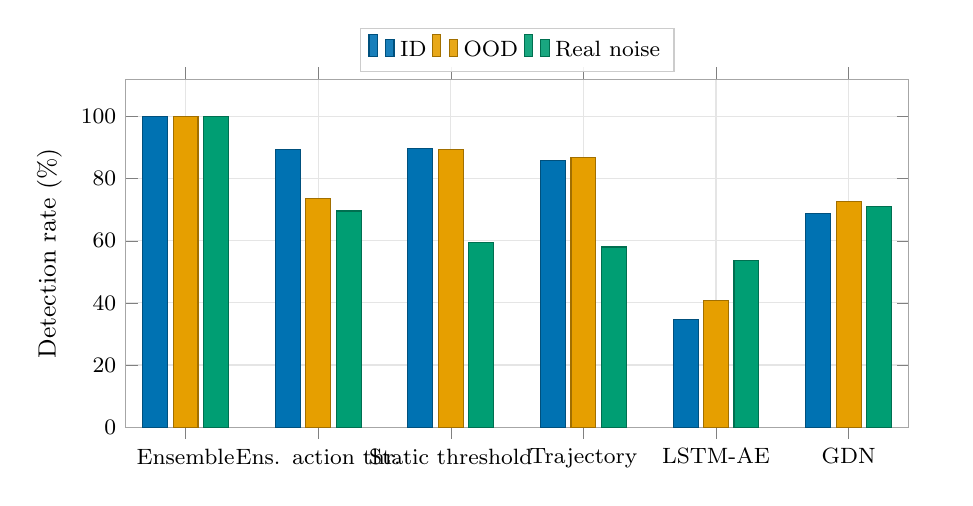
\begin{tikzpicture}
\begin{axis}[
  width=0.95\textwidth, height=60mm, ybar, bar width=9pt,
  symbolic x coords={Ensemble,Ens. action thr.,Static threshold,Trajectory,LSTM-AE,GDN},
  xtick=data, x tick label style={font=\footnotesize, align=center, text width=22mm},
  ylabel={Detection rate (\%)}, ymin=0, ymax=112, ytick={0,20,40,60,80,100},
  legend style={at={(0.5,1.02)}, anchor=south, legend columns=3},
  enlarge x limits=0.09,
]
\addplot[fill=oiblue, draw=oiblue!70!black] coordinates {(Ensemble,100) (Ens. action thr.,89.3) (Static threshold,89.8) (Trajectory,85.9) (LSTM-AE,34.6) (GDN,68.8)};
\addplot[fill=oiorange, draw=oiorange!70!black] coordinates {(Ensemble,100) (Ens. action thr.,73.5) (Static threshold,89.4) (Trajectory,86.7) (LSTM-AE,40.7) (GDN,72.6)};
\addplot[fill=oigreen, draw=oigreen!70!black] coordinates {(Ensemble,100) (Ens. action thr.,69.6) (Static threshold,59.4) (Trajectory,58.0) (LSTM-AE,53.6) (GDN,71.0)};
\legend{ID, OOD, Real noise}
\end{axis}
\end{tikzpicture}
\caption{Detection rate per method and test split at a 0.1\,\% false-positive target (data of
Table~\ref{tab:recall-lead}).}
\label{fig:recall-bars}
\end{figure}

\begin{figure}[ht]
\centering
\begin{minipage}[t]{0.49\textwidth}
\centering
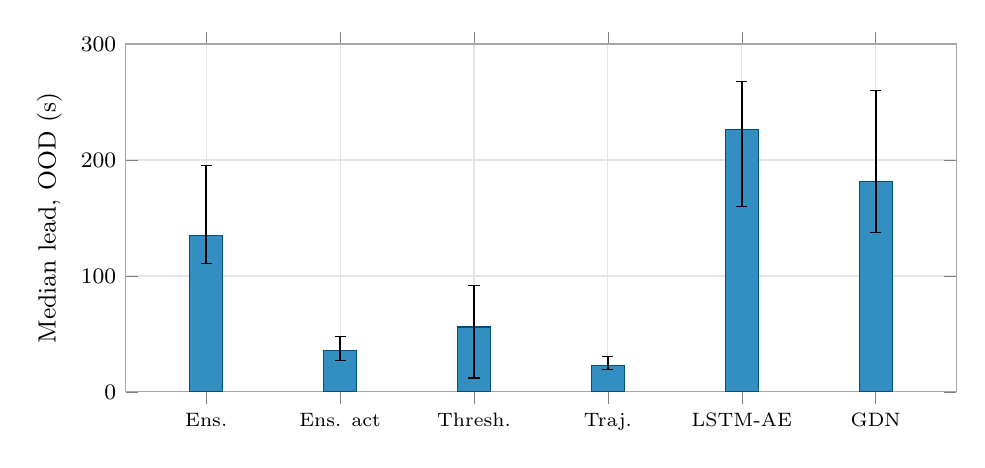
\begin{tikzpicture}
\begin{axis}[
  width=\linewidth, height=60mm, ybar, bar width=12pt,
  symbolic x coords={Ens.,Ens. act,Thresh.,Traj.,LSTM-AE,GDN},
  xtick=data, x tick label style={font=\scriptsize},
  ylabel={Median lead, OOD (s)}, ymin=0, ymax=300, enlarge x limits=0.12,
]
\addplot[fill=oiblue!80, draw=oiblue!70!black,
  error bars/.cd, y dir=both, y explicit, error bar style={black, thick}]
  coordinates {
  (Ens.,135) += (0,60) -= (0,24)
  (Ens. act,36) += (0,12) -= (0,9)
  (Thresh.,56) += (0,36) -= (0,44)
  (Traj.,23) += (0,7.75) -= (0,4)
  (LSTM-AE,226) += (0,41.75) -= (0,65.75)
  (GDN,181.5) += (0,78.5) -= (0,44.25)};
\end{axis}
\end{tikzpicture}
\caption{Median anticipation horizon on the OOD split; error bars span the IQR.}
\label{fig:lead-iqr}
\end{minipage}\hfill
\begin{minipage}[t]{0.49\textwidth}
\centering
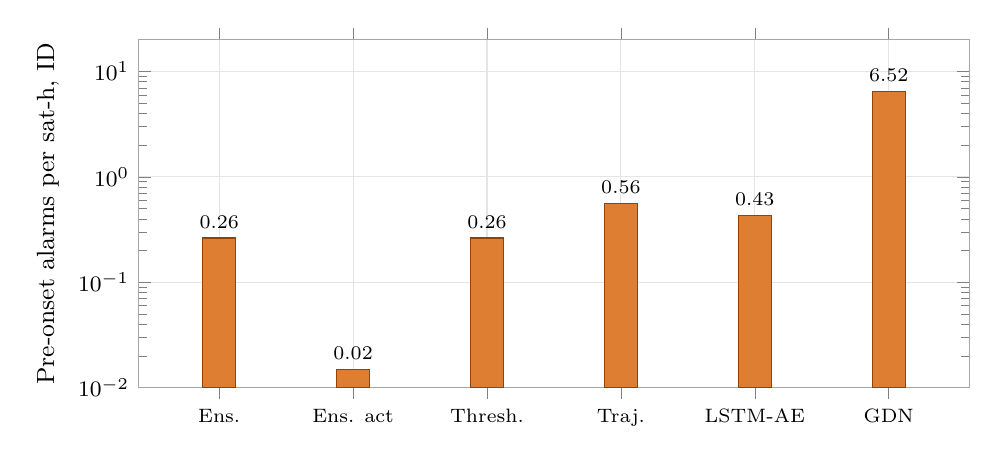
\begin{tikzpicture}
\begin{axis}[
  width=\linewidth, height=60mm, ybar, bar width=12pt, ymode=log, log origin=infty,
  symbolic x coords={Ens.,Ens. act,Thresh.,Traj.,LSTM-AE,GDN},
  xtick=data, x tick label style={font=\scriptsize},
  ylabel={Pre-onset alarms per sat-h, ID}, ymin=0.01, ymax=20, enlarge x limits=0.12,
  nodes near coords, nodes near coords style={font=\scriptsize},
  point meta=explicit symbolic,
]
\addplot[fill=oiverm!80, draw=oiverm!70!black] coordinates {
  (Ens.,0.263) [0.26] (Ens. act,0.015) [0.02] (Thresh.,0.263) [0.26] (Traj.,0.563) [0.56] (LSTM-AE,0.431) [0.43] (GDN,6.518) [6.52]};
\end{axis}
\end{tikzpicture}
\caption{False alarms raised before the attack onset (log scale).}
\label{fig:preonset}
\end{minipage}
\end{figure}

\subsection{Model convergence}
Fig.~\ref{fig:convergence} plots the training histories of the five released ensemble members
(\file{data/models/full\_s*.json}, release \texttt{models-v2}). Validation loss falls from 0.280 to
0.189 (mean of the members) over 8 epochs and the members agree within 0.010 at the last epoch, which
is what the ensemble's spread $Q$ relies on. An epoch takes about 110\,s on the laptop (median of the
recorded epoch times); training the five members and three ablations took 21\,min.

\begin{figure}[ht]
\centering
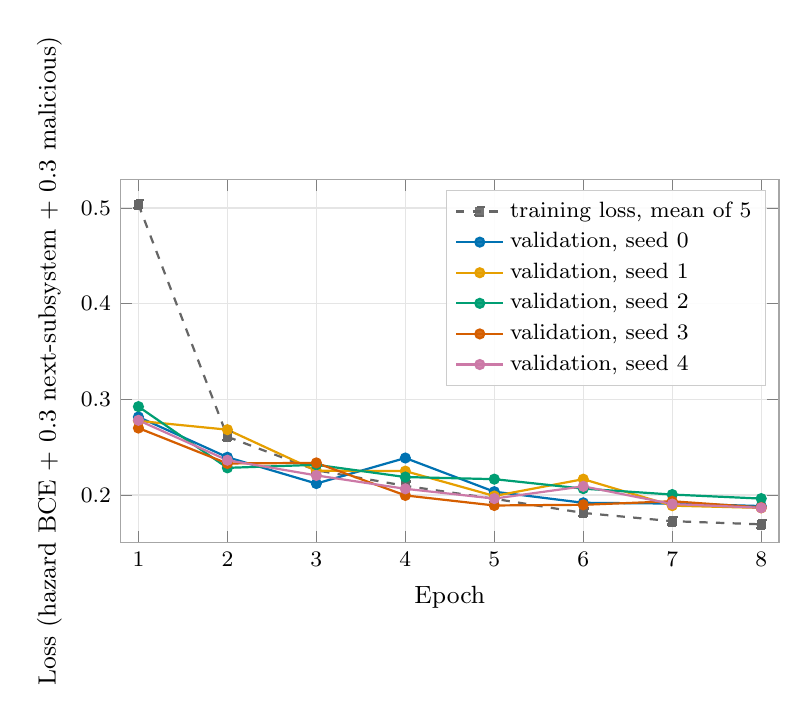
\begin{tikzpicture}
\begin{axis}[
  width=0.82\textwidth, height=62mm,
  xlabel={Epoch}, ylabel={Loss (hazard BCE + 0.3 next-subsystem + 0.3 malicious)},
  xmin=0.8, xmax=8.2, ymin=0.15, ymax=0.53, xtick={1,...,8},
  legend style={at={(0.98,0.97)}, anchor=north east},
]
\addplot[thick, dashed, oigrey, mark=square*, mark size=1.6pt] coordinates {(1,0.5036) (2,0.2609) (3,0.2259) (4,0.2096) (5,0.1961) (6,0.1813) (7,0.1727) (8,0.1694)};
\addlegendentry{training loss, mean of 5}
\addplot[thick, oiblue, mark=*, mark size=1.6pt] coordinates {(1,0.2816) (2,0.2395) (3,0.2120) (4,0.2387) (5,0.2035) (6,0.1919) (7,0.1911) (8,0.1885)};
\addlegendentry{validation, seed 0}
\addplot[thick, oiorange, mark=*, mark size=1.6pt] coordinates {(1,0.2775) (2,0.2683) (3,0.2254) (4,0.2250) (5,0.1990) (6,0.2166) (7,0.1889) (8,0.1866)};
\addlegendentry{validation, seed 1}
\addplot[thick, oigreen, mark=*, mark size=1.6pt] coordinates {(1,0.2924) (2,0.2284) (3,0.2316) (4,0.2188) (5,0.2166) (6,0.2067) (7,0.2005) (8,0.1963)};
\addlegendentry{validation, seed 2}
\addplot[thick, oiverm, mark=*, mark size=1.6pt] coordinates {(1,0.2700) (2,0.2330) (3,0.2336) (4,0.1996) (5,0.1891) (6,0.1898) (7,0.1935) (8,0.1870)};
\addlegendentry{validation, seed 3}
\addplot[thick, oipurple, mark=*, mark size=1.6pt] coordinates {(1,0.2781) (2,0.2364) (3,0.2205) (4,0.2065) (5,0.1963) (6,0.2091) (7,0.1906) (8,0.1867)};
\addlegendentry{validation, seed 4}
\end{axis}
\end{tikzpicture}
\caption{Convergence of the five ensemble members (training and validation loss per epoch).}
\label{fig:convergence}
\end{figure}

\subsection{Secondary heads and calibration}
\begin{table}[ht]
\centering
\caption{Calibration and secondary heads (\file{results/manifest.json} \texttt{headline}).}
\label{tab:heads}
\small
\begin{tabular}{@{}lccc@{}}
\toprule
Indicator & ID & OOD & Real noise \\
\midrule
ECE at 10\,s / 30\,s & 0.0007 / 0.0011 & 0.0002 / 0.0006 & 0.0001 / 0.0005 \\
ECE at 60\,s / 120\,s & 0.0021 / 0.0034 & 0.0016 / 0.0049 & 0.0008 / 0.0024 \\
Next affected subsystem, top-1 / top-3 & 0.856 / 0.996 & 0.833 / 0.993 & 0.244 / 0.819 \\
\quad samples & 3896 & 3626 & 2138 \\
Malicious vs fault, AUROC / accuracy & 0.954 / 0.897 & 0.941 / 0.906 & 0.936 / 0.868 \\
\quad samples & 22745 & 22193 & 10840 \\
\bottomrule
\end{tabular}
\end{table}

Calibration error stays below 0.005 at every horizon on every split (Table~\ref{tab:heads}), so a
forecast of $p$ can be read as a probability, which the uncertainty gate and the cost $\mathcal{J}(a)$
require. Attack-versus-fault discrimination holds under real noise; next-subsystem prediction does not
(top-1 drops to 0.24), and the dashboard therefore presents it as a prediction, never as an observation.

\subsection{Live closed-loop KPIs}
Table~\ref{tab:live} aggregates the live runs of the final configuration (attack at $t_a=60$\,s,
twin limit 45\,\degC). Detection delay $d$, response time $r$ and margin $m$ follow
Eq.~(\ref{eq:live}).

\begin{table}[ht]
\centering
\caption{Live runs, CASSANDRA in closed loop with the twin (min / median / max over runs). Sources:
\file{results/live\_manifest.json} (A1, A1 re-asserted, B1 seeds 1--3),
\file{results/phase6\_block3.json} (B1 seeds 4--6, C1 seeds 1--6, clean).}
\label{tab:live}
\small
\begin{tabular}{@{}lcccccc@{}}
\toprule
Scenario & Runs & Delay $d$ (s) & Response $r$ (s) & Margin $m$ (\degC) & Limit reached & False containm. \\
\midrule
A1 heater latch & 3 & 22 / 52 / 165 & 62 / 116 / 216 & 5.4 / 8.5 / 11.3 & 0 & 0 \\
A1 re-asserted commands & 3 & 5 / 10 / 50 & 43 / 84 / 203 & 9.0 / 10.6 / 16.0 & 0 & 0 \\
B1 telemetry masking & 6 & 8 / 8 / 8 & 55 / 71.5 / 79 & 5.4 / 10.7 / 19.9 & 0 & 0 \\
C1 cross-link relay (source) & 6 & 2 / 2 / 32 & 12 / 12 / 42 & 4.0 / 17.8 / 21.0$^{\dagger}$ & 0 & 0 \\
Clean operations & 3 & --- & --- & --- & 0 & 0 \\
\midrule
\textbf{All} & \textbf{21} & & & & \textbf{0} & \textbf{0} \\
\bottomrule
\end{tabular}

\smallskip
\footnotesize $^{\dagger}$Over every satellite of the C1 runs (sources and touched victims). Brief false
flags without action on non-attacked satellites: 6 in B1, 6 in C1, 1 in clean runs.
\end{table}

\begin{table}[ht]
\centering
\caption{Closed loop on the twin, 24 test episodes (\file{results/manifest.json} \texttt{closed\_loop},
\texttt{python -m eval.closed\_loop --episodes 24}). \textbf{Upper bound}: the planner uses the
simulator as its own model.}
\label{tab:closed}
\small
\begin{tabular}{@{}lr@{}}
\toprule
Failures averted & 13 of 18 (72.2\,\%; Wilson 49.1--87.5\,\%) \\
New failures caused by a response & 0 \\
Mean availability $A$ & 0.9989 \\
False containments & 1 (0.050 per orbital period) \\
Actions: safe mode / isolate subsystem & 13 / 11 \\
Decisions held by the uncertainty gate & 1 \\
\bottomrule
\end{tabular}
\end{table}

\subsection{Anticipation on the physical node}
Fig.~\ref{fig:board} compares, over time, the measured A1 run on the ESP8266 node with the trajectory
the same firmware model would follow without a response (computed: $+1.5$\,\degC/s from the measured
start temperature). A threshold alarm at the limit would fire only when the limit is reached
(23.2\,s by the model; Phase~2 measured 23.3\,s). CASSANDRA cut the heater at 20.0\,s in the bridge log, at a
peak of 54.36\,\degC, 5.6\,\degC{} below the limit; the dashboard received the flag 5.9\,s and the cut
21.9\,s after the attack command (\file{results/board\_a1.json}).

\begin{figure}[ht]
\centering
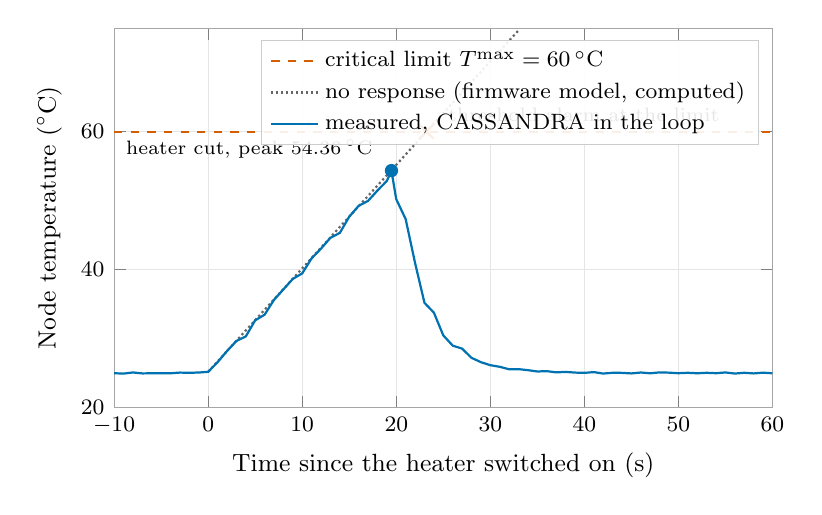
\begin{tikzpicture}
\begin{axis}[
  width=0.82\textwidth, height=64mm,
  xlabel={Time since the heater switched on (s)}, ylabel={Node temperature (\degC)},
  xmin=-10, xmax=60, ymin=20, ymax=75,
  legend style={at={(0.98,0.97)}, anchor=north east},
]
\addplot[thick, oiverm, dashed, domain=-10:60, samples=2] {60};
\addlegendentry{critical limit $T^{\max}=60$\,\degC}
\addplot[thick, oigrey, densely dotted, domain=0:33, samples=2] {25.19+1.5*x};
\addlegendentry{no response (firmware model, computed)}
\addplot[thick, oiblue] coordinates {
(-10,24.99) (-9,24.93) (-8,25.10) (-7,24.96) (-6,24.98) (-5,24.99) (-4,24.98) (-3,25.08) (-2,25.05)
(-1,25.09) (0,25.19) (1,26.58) (2,28.20) (3,29.66) (4,30.32) (5,32.66) (6,33.47) (7,35.62) (8,37.14)
(9,38.66) (10,39.46) (11,41.64) (12,43.05) (13,44.62) (14,45.33) (15,47.68) (16,49.25) (17,49.97)
(18,51.47) (19,52.87) (19.49,54.36) (19.99,50.24) (21,47.33) (22,40.96) (23,35.19) (24,33.77) (25,30.47)
(26,28.99) (27,28.55) (28,27.22) (29,26.59) (30,26.15) (31,25.92) (32,25.56) (33,25.58) (34,25.43)
(35,25.24) (36,25.29) (37,25.11) (38,25.18) (39,25.08) (40,25.04) (41,25.15) (42,24.94) (43,25.05)
(44,25.04) (45,24.96) (46,25.09) (47,24.98) (48,25.11) (49,25.07) (50,24.99) (51,25.05) (52,24.98)
(53,25.05) (54,24.99) (55,25.10) (56,24.94) (57,25.05) (58,24.96) (59,25.07) (60,24.98)};
\addlegendentry{measured, CASSANDRA in the loop}
\addplot[only marks, mark=*, mark size=2.2pt, oiblue] coordinates {(19.49,54.36)};
\addplot[only marks, mark=x, mark size=3.5pt, thick, oiverm] coordinates {(23.21,60)};
\node[font=\scriptsize, anchor=east] at (axis cs:18.5,57.5) {heater cut, peak 54.36\,\degC};
\node[font=\scriptsize, anchor=west] at (axis cs:24.5,62.5) {threshold alarm at the limit};
\end{axis}
\end{tikzpicture}
\caption{A1 on the physical node: measured temperature with the defence in the loop
(\file{results/board\_a1\_curve.csv}, one sample per second plus the exact peak) against the computed
no-response trajectory of the firmware model. Temperature emulated by the firmware.}
\label{fig:board}
\end{figure}

\subsection{Latency}
Fig.~\ref{fig:latency} plots, for each of the 26 recorded live runs, the median tick time and the median
planning time per decision against the 150\,ms budget; Table~\ref{tab:latency} gives the offline
measurements.

\begin{figure}[ht]
\centering
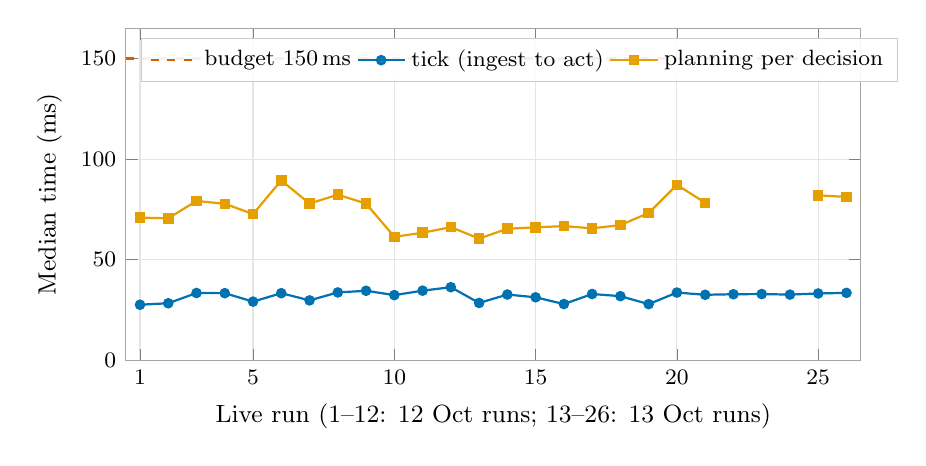
\begin{tikzpicture}
\begin{axis}[
  width=0.9\textwidth, height=58mm,
  xlabel={Live run (1--12: 12 Oct runs; 13--26: 13 Oct runs)},
  ylabel={Median time (\si{\milli\second})},
  xmin=0.5, xmax=26.5, ymin=0, ymax=165, xtick={1,5,10,15,20,25},
  legend style={at={(0.02,0.97)}, anchor=north west, legend columns=3},
]
\addplot[thick, oiverm, dashed, domain=0.5:26.5, samples=2] {150};
\addlegendentry{budget 150\,ms}
\addplot[thick, oiblue, mark=*, mark size=1.5pt] coordinates {(1,27.65) (2,28.39) (3,33.48) (4,33.39) (5,29.2) (6,33.38) (7,29.81) (8,33.76) (9,34.58) (10,32.43) (11,34.63) (12,36.36) (13,28.53) (14,32.71) (15,31.34) (16,27.98) (17,32.97) (18,31.9) (19,27.94) (20,33.69) (21,32.59) (22,32.86) (23,32.95) (24,32.68) (25,33.24) (26,33.54)};
\addlegendentry{tick (ingest to act)}
\addplot[thick, oiorange, mark=square*, mark size=1.5pt] coordinates {(1,70.9) (2,70.6) (3,79.2) (4,77.8) (5,72.7) (6,89.4) (7,77.9) (8,82.3) (9,77.9) (10,61.4) (11,63.4) (12,66.2) (13,60.5) (14,65.4) (15,66.1) (16,66.7) (17,65.6) (18,67.2) (19,73.2) (20,87.2) (21,78.3)};
\addlegendentry{planning per decision}
\addplot[thick, oiorange, mark=square*, mark size=1.5pt, forget plot] coordinates {(25,82.0) (26,81.2)};
\end{axis}
\end{tikzpicture}
\caption{Per-run latency of the live core with the ensemble (\file{results/live\_manifest.json},
\file{results/phase6\_block3.json}). Runs 22--24 are clean runs: no decision, so no planning time.}
\label{fig:latency}
\end{figure}

\begin{table}[ht]
\centering
\caption{Offline timing on the x86 laptop (\file{results/manifest.json} \texttt{latency},
\texttt{closed\_loop}).}
\label{tab:latency}
\small
\begin{tabular}{@{}lr@{}}
\toprule
Ensemble inference, 5 models, 1 thread, median / p95 & 17.6 / 20.9\,ms \\
Ensemble inference, 5 models, 4 threads, median / p95 & 21.9 / 40.0\,ms \\
Offline evaluator, step median & 22.4\,ms \\
Offline evaluator planning, median / p95 & 254 / 402\,ms \\
\bottomrule
\end{tabular}
\end{table}

% =====================================================================================================
\section{Constraint and Stress-Testing Evaluation}
\label{sec:stress}

\subsection{Edge conditions}
Table~\ref{tab:edge} lists every degraded condition we evaluated and, explicitly, the ones we did not.

\begin{table}[ht]
\centering
\caption{Degraded and adversarial conditions.}
\label{tab:edge}
\small
\begin{tabular}{@{}>{\raggedright\arraybackslash}p{0.30\textwidth}>{\raggedright\arraybackslash}p{0.45\textwidth}>{\raggedright\arraybackslash}p{0.18\textwidth}@{}}
\toprule
Condition & Result & Source \\
\midrule
Real operational noise and telemetry gaps (OPS-SAT) & ensemble DR 1.00, lead 158\,s; static threshold falls to 0.59, trajectory to 0.58 & manifest \texttt{headline} \\
Unseen generator families (OOD) & ensemble DR 1.00, lead 135\,s; no-engineered-features ablation falls to 0.90 & manifest \texttt{headline} \\
Adversarial perturbation of housekeeping telemetry, $\varepsilon\le 1$ nominal std. & ensemble DR 0.75--1.00, mean $Q$ rises 0.087 $\rightarrow$ 0.207 (Fig.~\ref{fig:robust}); threshold DR 0.83 & manifest \texttt{robustness} (12 episodes) \\
Spoofed ground origin on every command & DR 1.00, lead 134\,s & manifest \texttt{stress} \\
No telecommand evidence at all & DR 1.00, lead 133\,s & manifest \texttt{stress} \\
Forged telemetry (B1, live) & monitor confirms 8\,s after the attack in all 6 runs; no limit reached & live runs \\
Repeated malicious commands (A1 re-asserted, live) & escalation to safe mode, which refuses them; healed after the attack stops & live runs \\
Propagation over feasible ISLs (C1, live) & source quarantined in 6/6 runs, 12--42\,s; no victim at its limit & block 3 runs \\
Battery drain attack (A3, offline) & DR 1.00, lead 244\,s & manifest \texttt{stress} \\
Higher plant speed (20$\times$, ensemble, through the broker) & tick median 47.9\,ms, p95 60.3\,ms; use $\le$10$\times$ live & \file{docs/STATUS.md} \\
Total communication loss & \textbf{not measured} (ingest marks values stale after 3\,s) & --- \\
Degraded battery as a standing condition & \textbf{not measured separately} (F3 ageing is part of the benign set behind the FPR) & --- \\
Compute or thermal throttling of the ground station & \textbf{not measured} & --- \\
\bottomrule
\end{tabular}
\end{table}

\subsection{Robustness to telemetry perturbation}
Fig.~\ref{fig:robust} shows the projected-gradient attack on the forgeable housekeeping channels. The
ensemble's detection rate dips to 0.75 at $\varepsilon=0.25$ and recovers at larger budgets, a
non-monotonic curve that reflects the small sample (12 episodes). Two properties matter more for
operations: the static threshold's lead shrinks from 40.5 to 23.5\,s as $\varepsilon$ grows, and the
ensemble's mean uncertainty $Q$ more than doubles, so a stronger forgery pushes more decisions towards
the uncertainty gate (safe hold and ground alert) rather than towards autonomous isolation.

\begin{figure}[ht]
\centering
\begin{minipage}[t]{0.49\textwidth}
\centering
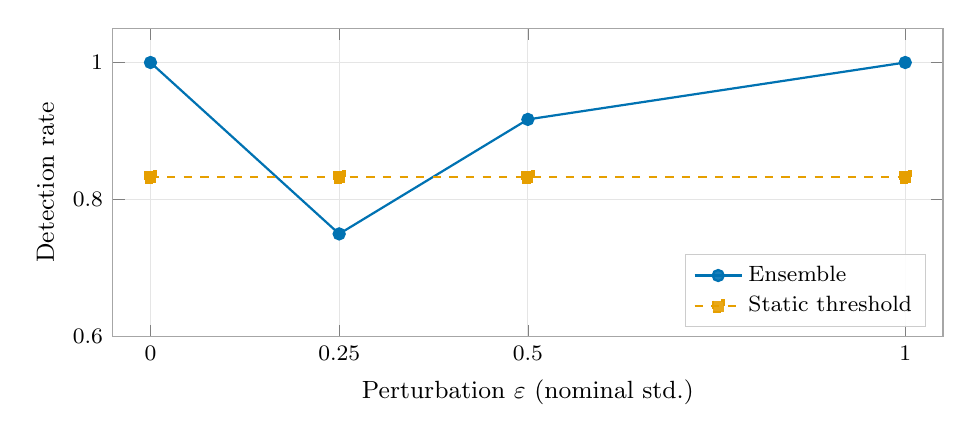
\begin{tikzpicture}
\begin{axis}[
  width=\linewidth, height=55mm,
  xlabel={Perturbation $\varepsilon$ (nominal std.)}, ylabel={Detection rate},
  xmin=-0.05, xmax=1.05, ymin=0.6, ymax=1.05, xtick={0,0.25,0.5,1},
  legend style={at={(0.98,0.03)}, anchor=south east},
]
\addplot[thick, oiblue, mark=*] coordinates {(0,1.000) (0.25,0.750) (0.5,0.917) (1,1.000)};
\addlegendentry{Ensemble}
\addplot[thick, dashed, oiorange, mark=square*] coordinates {(0,0.833) (0.25,0.833) (0.5,0.833) (1,0.833)};
\addlegendentry{Static threshold}
\end{axis}
\end{tikzpicture}
\end{minipage}\hfill
\begin{minipage}[t]{0.49\textwidth}
\centering
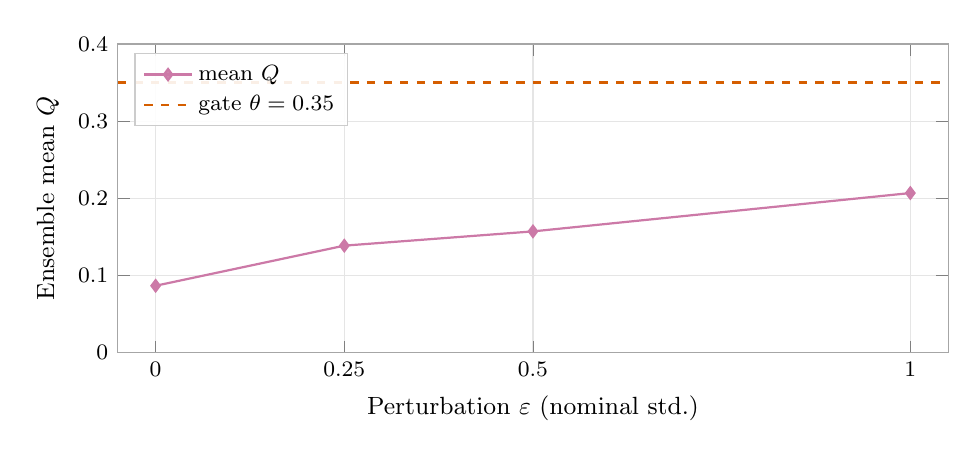
\begin{tikzpicture}
\begin{axis}[
  width=\linewidth, height=55mm,
  xlabel={Perturbation $\varepsilon$ (nominal std.)}, ylabel={Ensemble mean $Q$},
  xmin=-0.05, xmax=1.05, ymin=0, ymax=0.4, xtick={0,0.25,0.5,1},
  legend style={at={(0.02,0.97)}, anchor=north west},
]
\addplot[thick, oipurple, mark=diamond*] coordinates {(0,0.0866) (0.25,0.1386) (0.5,0.1571) (1,0.2068)};
\addlegendentry{mean $Q$}
\addplot[thick, oiverm, dashed, domain=-0.05:1.05, samples=2] {0.35};
\addlegendentry{gate $\theta=0.35$}
\end{axis}
\end{tikzpicture}
\end{minipage}
\caption{Robustness to a projected-gradient attack on housekeeping telemetry
(\file{results/manifest.json} \texttt{robustness}, \texttt{python -m eval.robustness --episodes 12}).
Left: detection rate. Right: ensemble uncertainty against the gate threshold.}
\label{fig:robust}
\end{figure}

\subsection{Cyber-evidence stress test}
\begin{table}[ht]
\centering
\caption{Median lead (s) per attack type on the ID split with all failing satellites detected in every
variant (\file{results/manifest.json} \texttt{stress}, \texttt{python -m eval.stress}; 140 attack
episodes, 183 failing satellites).}
\label{tab:stress}
\small
\begin{tabular}{@{}lccccccc@{}}
\toprule
Variant & A1 & A2 & A3 & B1 & B2 & C1 & All \\
\midrule
Original telecommands & 125 & 139 & 244 & 186 & 156 & 126 & 135 \\
Every origin spoofed as ground & 125 & 139 & 244 & 186 & 156 & 126 & 134 \\
No telecommands at all & 125 & 133 & 244 & 186 & 155 & 126 & 133 \\
\midrule
Failing satellites & 28 & 31 & 16 & 15 & 14 & 79 & 183 \\
\bottomrule
\end{tabular}
\end{table}

Removing or spoofing the command evidence changes the lead by at most 6\,s (Table~\ref{tab:stress}):
on this benchmark the physical channels alone are enough to detect every failure. This makes the system
robust to an attacker who hides the command channel, but it also means the benchmark cannot show what
the cyber features add (Section~\ref{sec:ablation}).

% =====================================================================================================
\section{Trade-off and Ablation Study}
\label{sec:ablation}

\subsection{Model ablations}
\begin{table}[ht]
\centering
\caption{Model ablations: detection rate / median lead (s) (\file{results/manifest.json}
\texttt{headline}).}
\label{tab:ablation}
\small
\begin{tabular}{@{}lccc@{}}
\toprule
Variant & ID & OOD & Real noise \\
\midrule
Full ensemble (5 members) & 1.000 / 133 & 1.000 / 135 & 1.000 / 158 \\
Single member & 1.000 / 133 & 1.000 / 138 & 1.000 / 164 \\
No engineered features (no $E_{\mathrm{eng}}$) & 1.000 / 132 & \textbf{0.903} / 134.5 & 1.000 / 156 \\
No physical residual $\Delta\Phi$ & 1.000 / 133 & 1.000 / 142 & 1.000 / 167 \\
Unconstrained graph (all intra-satellite edges) & 1.000 / 134 & 1.000 / 135 & 1.000 / 158 \\
\bottomrule
\end{tabular}
\end{table}

\textbf{Reading the ablations honestly.} Every variant except one reaches a detection rate of 1.00 on
every split (Table~\ref{tab:ablation}); the benchmark saturates. The single informative difference is
that removing the engineering edges costs 10 points of recall on the out-of-distribution split. The
ensemble's value is not recall but the uncertainty $Q$ that the safety gate needs; a single member
gives no $Q$, and the gate is then reported as inactive.

\subsection{Operating-point trade-off: warning versus acting}
The same forecaster serves two thresholds. Alerting at $\tau=0.0153$ maximises the anticipation
horizon; acting at $\bar p\ge 0.5$ avoids responses to low-probability alerts.

\begin{table}[ht]
\centering
\caption{Alert level versus action threshold, same model (\file{results/manifest.json}
\texttt{headline}, \texttt{ensemble} and \texttt{ensemble@act}).}
\label{tab:operating}
\small
\begin{tabular}{@{}llcccc@{}}
\toprule
Split & Threshold & DR & Median lead (s) & FPR (\%) & $\lambda_{\mathrm{pre}}$ (per sat-h) \\
\midrule
\multirow{2}{*}{ID} & alert $\tau=0.0153$ & 1.000 & 133 & 0.150 & 0.26 \\
 & act $0.5$ & 0.893 & 38 & 0.008 & 0.02 \\
\multirow{2}{*}{OOD} & alert $\tau$ & 1.000 & 135 & 0.084 & 0.33 \\
 & act $0.5$ & 0.735 & 36 & 0.000 & 0.00 \\
\multirow{2}{*}{Real noise} & alert $\tau$ & 1.000 & 158 & 0.152 & 0.44 \\
 & act $0.5$ & 0.696 & 39.5 & 0.002 & 0.00 \\
\bottomrule
\end{tabular}
\end{table}

Raising the threshold from $\tau$ to 0.5 divides the false-positive rate by about 19 on the ID split
(and brings it to 0.000--0.002\,\% on the others) and the pre-onset alarm rate by about 17, at the
price of 95--119\,s of anticipation and 11--30 points of recall (Table~\ref{tab:operating}). The design uses both: operators see the early warning, and the autonomous
response waits for a likely failure.

\subsection{Decision-parameter ablations in closed loop}
\begin{table}[ht]
\centering
\caption{Ablations of response parameters, live runs (sources in each row).}
\label{tab:decision}
\small
\begin{tabular}{@{}>{\raggedright\arraybackslash}p{0.25\textwidth}>{\raggedright\arraybackslash}p{0.33\textwidth}>{\raggedright\arraybackslash}p{0.33\textwidth}@{}}
\toprule
Parameter & Setting A & Setting B (deployed) \\
\midrule
Heating rate used to estimate an untrusted temperature (B1, seeds 1--3) & 0.2\,\degC/s: responses at 124 / 94 / 124\,s; peaks 45.32 / 37.19 / 29.23\,\degC; \textbf{limit crossed in seed 1} (\file{live\_manifest\_heat0.2.json}) & 0.3\,\degC/s: responses at 75 / 55 / 75\,s; peaks 36.54 / 32.10 / 25.12\,\degC; no limit reached (\file{live\_manifest.json}) \\
Future-victim term in $R$ (C1, seeds 1--6) & off: source contained 5/6 (37--137\,s, median 57\,s); 10 victims touched (\file{phase6\_c1\_prefix.json}) & on: source contained 6/6 (12--42\,s, median 12\,s); 6 victims touched (\file{phase6\_block3.json}) \\
Decision rule for the physical node (A1, dry run, firmware model) & $\bar p(t,60\,\mathrm{s})\ge 0.5$: action $\approx$2\,s after the latch at 28.6\,\degC{} (\file{docs/STATUS.md}) & $\hat p(t,30\,\mathrm{s})\ge 0.85$: heater cut $\approx$19\,s after the command at 54.0\,\degC{} (\file{board\_rule\_dryrun.txt}) \\
Inference threads (offline) & 1 thread: 17.6 / 20.9\,ms & 4 threads: 21.9 / 40.0\,ms (no gain on this laptop) \\
\bottomrule
\end{tabular}
\end{table}

\begin{figure}[ht]
\centering
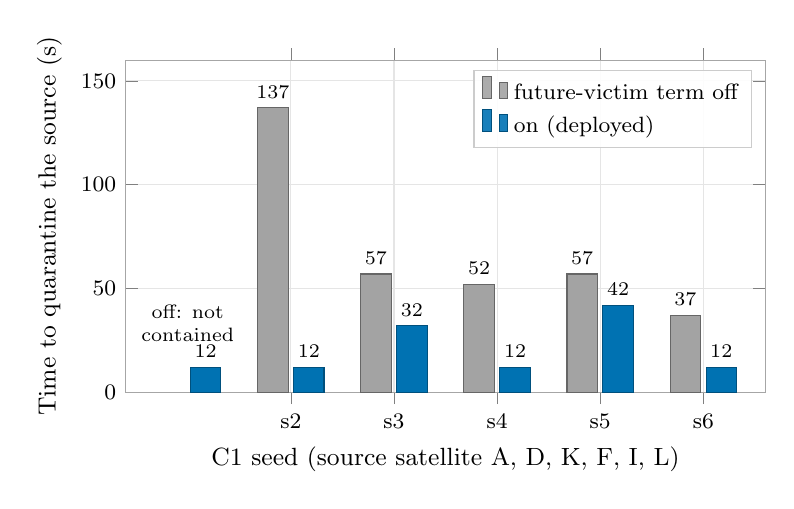
\begin{tikzpicture}
\begin{axis}[
  width=0.8\textwidth, height=58mm, ybar, bar width=11pt,
  symbolic x coords={s1,s2,s3,s4,s5,s6}, xtick=data,
  xlabel={C1 seed (source satellite A, D, K, F, I, L)}, ylabel={Time to quarantine the source (s)},
  ymin=0, ymax=160, enlarge x limits=0.12,
  legend style={at={(0.98,0.97)}, anchor=north east},
  nodes near coords, nodes near coords style={font=\scriptsize},
]
\addplot[fill=oigrey!60, draw=oigrey] coordinates {(s2,137) (s3,57) (s4,52) (s5,57) (s6,37)};
\addlegendentry{future-victim term off}
\addplot[fill=oiblue, draw=oiblue!70!black] coordinates {(s1,12) (s2,12) (s3,32) (s4,12) (s5,42) (s6,12)};
\addlegendentry{on (deployed)}
\node[font=\scriptsize, anchor=south, align=center] at (axis cs:s1,20) {off: not\\contained};
\end{axis}
\end{tikzpicture}
\caption{Effect of counting future relay victims in the response cost (\file{results/phase6\_c1\_prefix.json}
versus \file{results/phase6\_block3.json}).}
\label{fig:c1}
\end{figure}

\subsection{Where the approach succeeds and where trade-offs remain}
\begin{itemize}
\item \textbf{Succeeds.} Early warning with a controlled false-positive rate on unseen generator
families and real noise; calibrated probabilities; masking exposed within the monitor window; safe
mode that defeats re-asserted commands without knowing they are malicious; containment of a
propagating attack at its source; no false containment and no limit reached in 21 live runs (18
attacks, 3 clean); per-tick
latency well inside the budget.
\item \textbf{Trade-offs.} Acting late enough to avoid false responses costs anticipation (about 36--40\,s
of lead at the action threshold instead of 133--158\,s). The node rule trades margin (5.6\,\degC) for a
visible climb. The ensemble costs five forward passes for an uncertainty estimate. Quarantined C1
sources stay out of service until ground clears them (by design).
\item \textbf{Open evidence gaps.} The synthetic benchmark saturates, so the value of the graph
structure and cyber features is not measured; closed-loop numbers are an upper bound; next-subsystem
prediction degrades under real noise; latency on the Raspberry~Pi target, total communication loss and
energy consumption are not measured; the node's temperature is emulated by firmware.
\end{itemize}

\bibliographystyle{IEEEtran}
\bibliography{references}

\end{document}
